%\documentclass{amsart}

\documentclass{article}
\usepackage[letterpaper,hmargin=15mm,vmargin=20mm]{geometry}
\usepackage[nosetup, colorlinks]{tony}
\usepackage{graphicx}

\usepackage{amsmath,amssymb}
\usepackage{siunitx}

\usepackage{mathpazo}
\usepackage{microtype}
\usepackage{multicol}

\usepackage{diagbox}

\usepackage{color}
\usepackage[dvipsnames]{xcolor}
%\usepackage[printwatermark]{xwatermark}
%\newwatermark*[allpages,color=gray!50,angle=45,scale=3,xpos=0,ypos=0]{DRAFT}

\usepackage{tikz}
\usetikzlibrary{arrows}

\DeclareMathOperator{\sgn}{sgn}
\DeclareMathOperator{\NLL}{NLL}
\newcommand{\sind}[1]{^{(#1)}}

\title{6.867: Problem Set 3}
\date{November 10, 2016}

\begin{document}
\maketitle

\begin{multicols}{2}

% % % % % % % % % %
%    PROBLEM 1
% % % % % % % % % %

\section{Neural Networks}
\label{sec:nn}

\def\layersep{2.5cm}

\begin{figure*}[t]
    \label{fig:samplenn}
    \centering
    % tikz taken and adjusted from
% http://www.texample.net/tikz/examples/neural-network/
\begin{tikzpicture}[shorten >=1pt,->,draw=black!50, node distance=\layersep]
        \tikzstyle{every pin edge}=[<-,shorten <=1pt]
        \tikzstyle{neuron}=[circle,fill=black!25,minimum size=16pt,inner sep=0pt]
        \tikzstyle{input neuron}=[neuron, fill=CornflowerBlue!50];
        \tikzstyle{output neuron}=[neuron, fill=Dandelion!50];
        \tikzstyle{hidden neuron}=[neuron, fill=YellowGreen!50];
        \tikzstyle{annot} = [text width=5em, text centered]
    
        % Draw the input layer nodes
        \foreach \name / \y in {1,...,2}
        % This is the same as writing \foreach \name / \y in {1/1,2/2,3/3,4/4}
            \node[input neuron, pin=left:Input \#\y] (I-\name) at (0,-1cm-\y cm) {};
    
        % Draw the hidden layer nodes
        \foreach \name / \y in {1,...,5}
            \path[yshift=0.5cm]
                node[hidden neuron] (H-\name) at (\layersep,-\y cm) {};
                
        \foreach \name / \y in {6,...,10}
            \path[yshift=0.5cm]
                node[hidden neuron] (H-\name) at (2*\layersep,-\y cm + 5cm) {};
    
        % Draw the output layer node
        \foreach \name / \y in {1,...,3}
            \node[output neuron,pin={[pin edge={->}]right:Output \#\y}, right of=H-8] (O-\name) at (2*\layersep, -\y cm-0.5cm){};
    
        % Connect every node in the input layer with every node in the
        % hidden layer.
        \foreach \source in {1,...,2}
            \foreach \dest in {1,...,5}
                \path (I-\source) edge (H-\dest);
        
        % Connect every node in hidden layer 1 to hidden layer 2
        \foreach \source in {1,...,5}
            \foreach \dest in {6,...,10}
                \path (H-\source) edge (H-\dest);
    
        % Connect every node in the hidden layer with the output layer
        \foreach \source in {6,...,10}
            \foreach \dest in {1,...,3}
                \path (H-\source) edge (O-\dest);
    
        % Annotate the layers
        \node[annot,above of=H-1, node distance=1cm] (hl) {Hidden layer (ReLU)};
        \node[annot,left of=hl] {Input layer};
        \node[annot,right of=hl] (hl2) {Hidden layer (ReLU)};
        \node[annot,right of=hl2] {Output layer (softmax)};
\end{tikzpicture}

    \caption{Topology of a fully-connected neural network, with 2D inputs and 3-class outputs.}
\end{figure*}

We implemented a traditional, fully-connected neural network,
with arbitrary user-specified architecture.
We trained the neural network
through stochastic gradient descent on our data,
where gradients were calculated by the
backpropagation algorithm.

All hidden units were implemented with ReLU activation functions,
defined as
\begin{equation}
    f(z) = \max(0, z).
\end{equation}
% Describe how the choice of a softmax output layer and 
% cross-entropy loss is incorporated into your implementation.
The output layer was implemented as a softmax layer for $k$ classes.
Its activation function is given as the vector $f(z)$ where
\begin{equation}
    f(z)_i = \f{e^{z_i}}{\sum_{j=1}^{k}{e^{z_j}}} \tx{ for } i = 1,\dots,k.
\end{equation}
The softmax function separates classes
by assigning higher values to more likely classes,
so for a given sample $x$, we estimate its class $y$ as the most likely one
given by softmax.
We took target vectors of ``one-hot'' (1-of-$k$) vectors,
whose loss we measured with cross-entropy.
For a given training point $(x,y)$, the loss is
\begin{equation}
    l = \sum_{i = 1}^k{y_i \log(f(z)_i)}
\end{equation}
where $f(z)$ is defined above as the softmax output.
In the backpropagation algorithm,
we calculated the output layer loss using
the cross-entropy of the softmax function,
\begin{equation}
    \delta^L = f'(z^L)\circ\nabla_{a^L}l = f(z^L) - y
\end{equation}
where $\circ$ is element-wise multiplication, $f(z^L)$ is the softmax output,
and $y$ is the target vector.
This cross-entropy loss is backpropagated through the
loss calculations for the hidden layers,
which utilize the ReLU gradient instead.

We tested our neural network on a 2D 3-class dataset,
partitioned into 400 training, 200 validation, and 200 testing samples.
We show a possible topology for this neural network
in Figure~\ref{fig:samplenn}.

Neural network performance was very sensitive to
variations in weight initialization and step size.
For example, bad step sizes often resulted in
the network predicting only a single value for all inputs.

\begin{figure*}
   \centering
   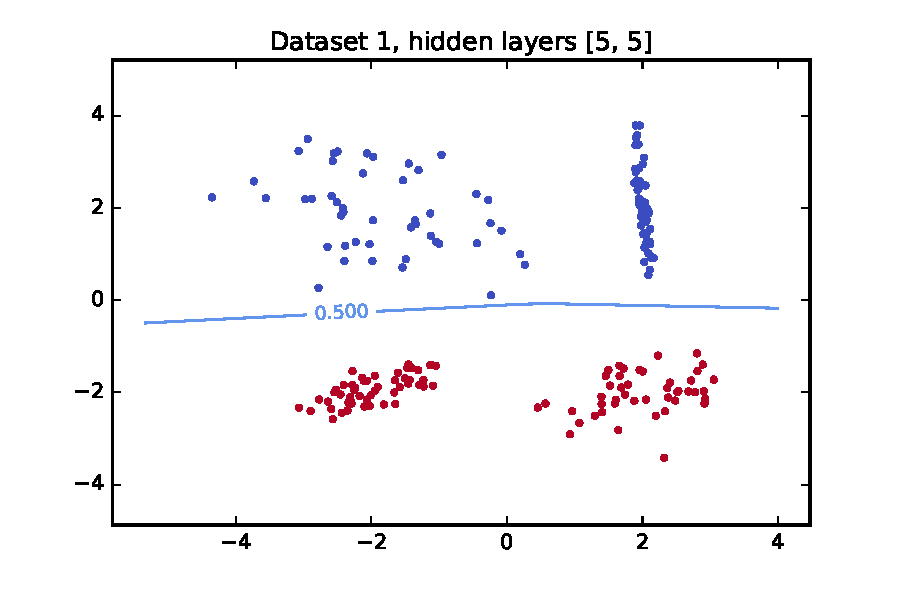
\includegraphics[width=3in]{img/p1/1-200of200.pdf}\hspace{-.25in}
   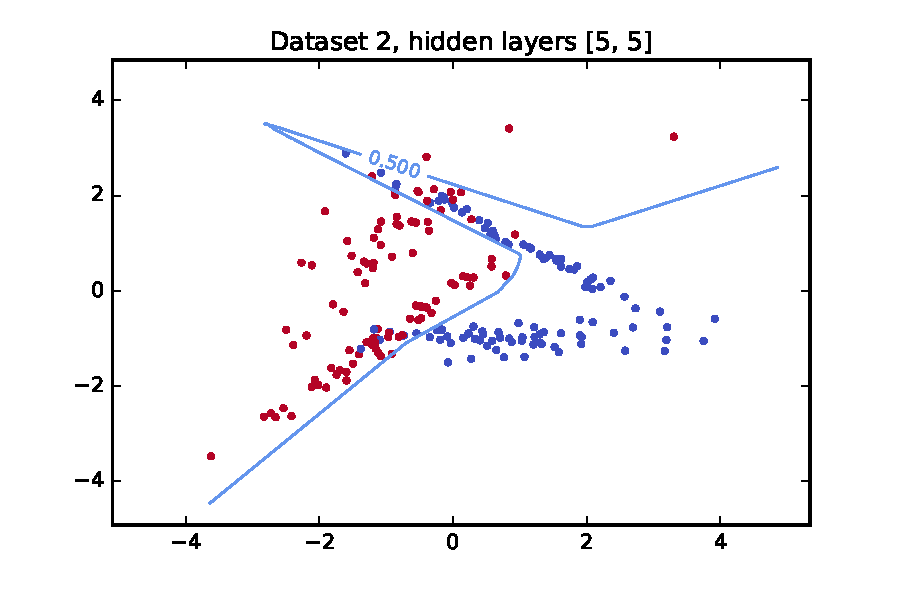
\includegraphics[width=3in]{img/p1/2-183of200.pdf}
   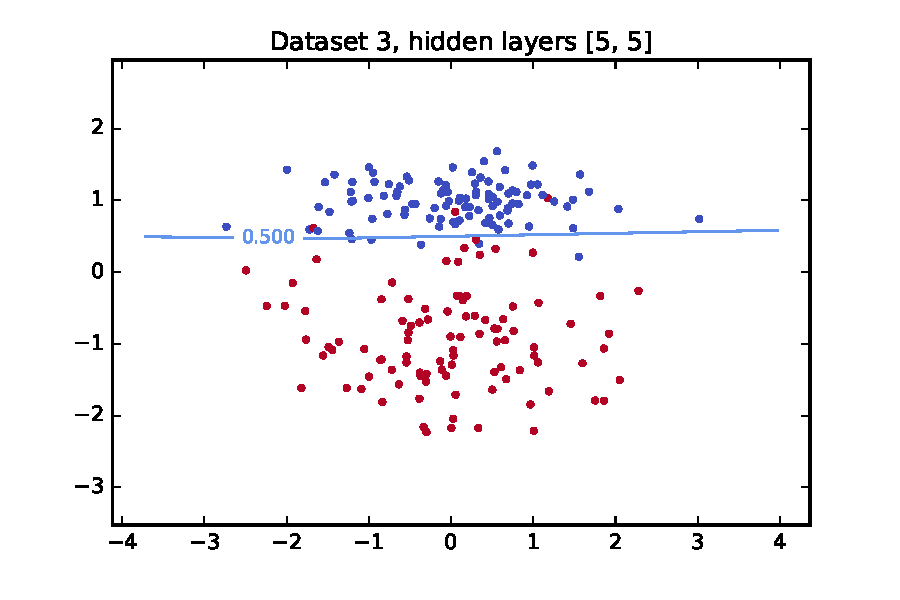
\includegraphics[width=3in]{img/p1/3-192of200.pdf}\hspace{-.25in}
   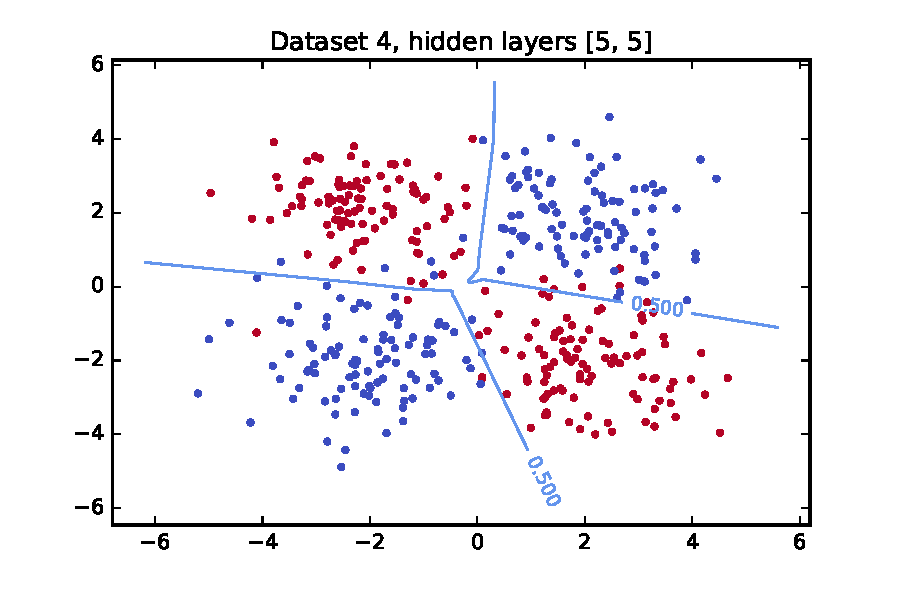
\includegraphics[width=3in]{img/p1/4-382of400.pdf}
   \caption{Neural network classification of four 2D datasets.
   Datasets 1-4 had training/testing accuracies 1.0/1.0, 0.9375/0.915, 0.9825/0.965, and 0.96/0.955,
   respectively.
   }
   \label{fig:1-2-classify}
\end{figure*}

\begin{figure*}
   \centering
   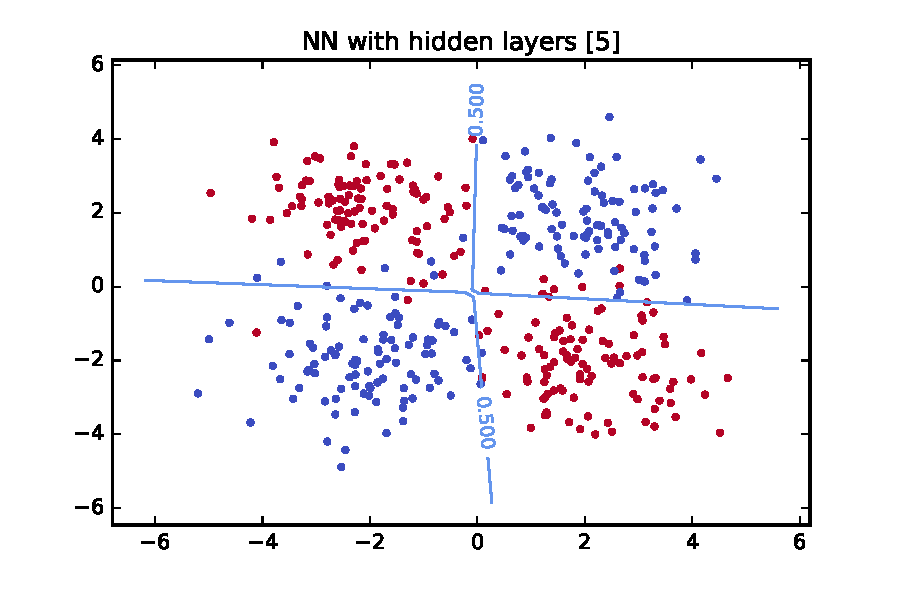
\includegraphics[width=3in]{img/p1/4-1small-382of400-16500.pdf}\hspace{-.25in}
   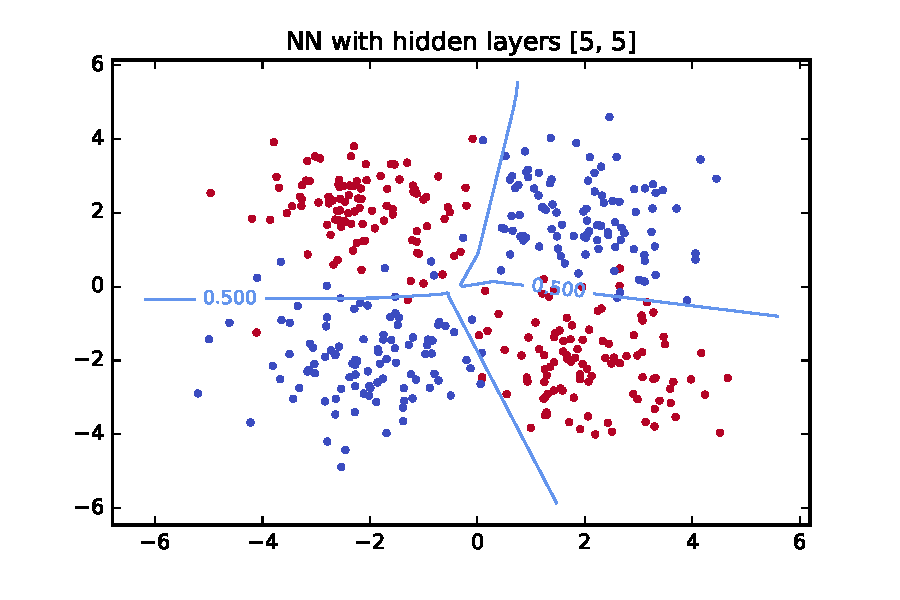
\includegraphics[width=3in]{img/p1/4-2small-380of400-3550.pdf}
   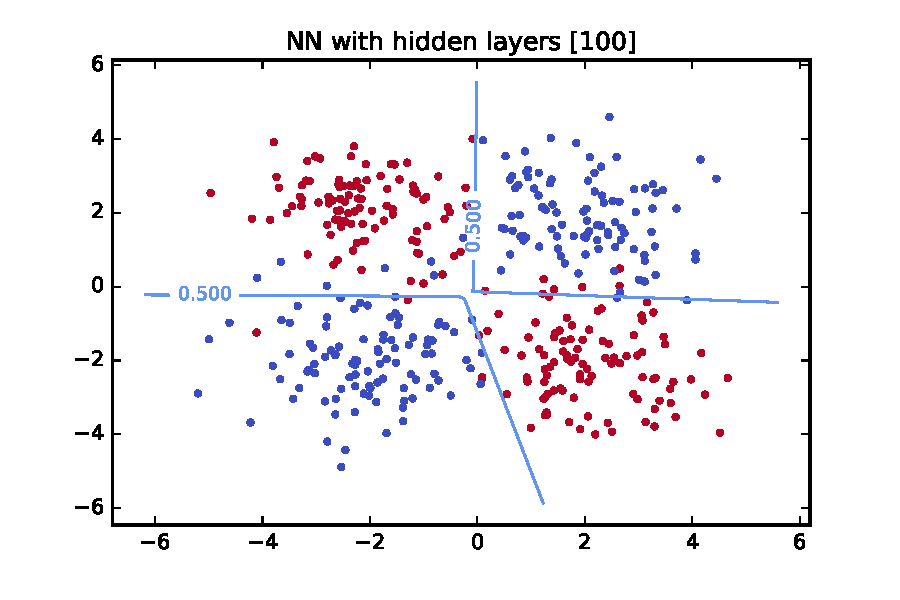
\includegraphics[width=3in]{img/p1/4-1large-380of400.pdf}\hspace{-.25in}
   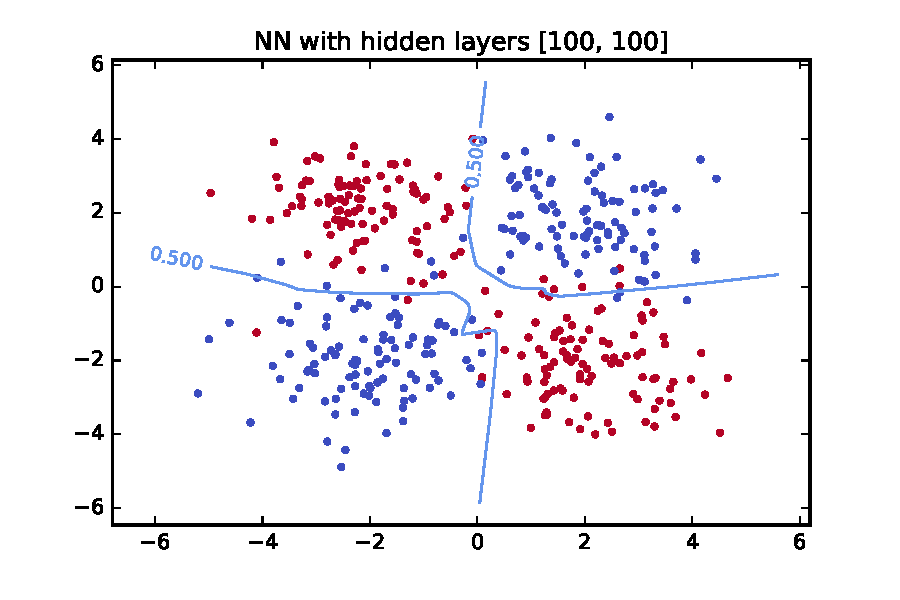
\includegraphics[width=3in]{img/p1/4-2large-379of400-123000.pdf}
   \caption{Variations on neural network architectures for classification of
   XOR data. We see that increasing number of layers increases non-linearity,
   while increasing number of nodes per layer increases overfitting. 
   }
   \label{fig:1-2-arch}
\end{figure*}

\subsection{Network training}

We stochastically updated our weights,
by randomly selecting a sample $(x^{(i)}, y^{(i)})$ per epoch
and updating accordingly.
Our update function is as follows,
\begin{align}
W_{t+1} &= W_t - \eta \f{\partial l}{\partial W_t^l}
= W_t - \eta a^{l-1} (\delta^l)^T \\
b_{t+1} &= b_t - \eta \f{\partial l}{\partial b_t^l}
= b_t - \eta \delta^l
\end{align}
where $l$ is cross-entropy loss, $\eta$ is the learning rate,
and $\delta$ is the calculated backpropagation error.

\subsubsection{Initialization}

Since ReLU is not fully differentiable,
we set the subgradient at 0 to 0.
As a result, we cannot simply initialize weights to 0;
otherwise gradients and activations
will not be updated during training.
Instead, we initialize weights randomly.
For a weight matrix of size $m\times n$,
draw values from a Gaussian centered at 0,
with standard deviation $1/\sqrt{m}$.

To understand the rationale behind this method,
imagine that all units are sigmoids,
with activation $f(z) = \f{1}{1+e^{-z}}$.
If weights are too small,
activations will become miniscule in shallower layers,
which is an issue since the sigmoid function
is approximately linear around 0,
at which we lose the non-linearity of our hidden layers.

However, if our weights are too large,
activations will grow indefinitely.
The sigmoid levels off for large inputs,
so gradients artificially approach 0.
Thus, we want to maintain a constant variance in gradients between
inputs and outputs, such that
\begin{equation}
\f{\sigma^2(z)}{\sigma^2(x)} = \f{\sigma^2(W^TX)}{\sigma^2(X)}
= \f{n\sigma^2(W)\sigma^2{X}}{\sigma^2(X)} = n\sigma^2(W) = 1
\end{equation}
For backpropagation, we use the same logic to derive that
$\sigma^2(W) = 1/m$, so $\sigma(W) = 1/\sqrt{m}$.

\subsubsection{Regularization}
\label{subsubsec:1-regularize}

To avoid overfitting, we can add a penalty term to our loss function for regularization.
Our loss would thus become
\begin{equation}
    J(w) = l(w) +
      \lambda
        \lt(\lVert w^{(1)} \rVert^2_F + \lVert w^{(2)} \rVert^2_F\rt)
\end{equation}
where $\lVert w\rVert = \sqrt{\sum_{i,j}{w_{ij}^2}}$ is the Frobenius norm.
In particular, the regularization term is added to the output error $\delta^L$
during backpropagation. The change in $\delta^L$ is then propagated
through to subsequent error calculations for each hidden layer
(even though we don't compute the error again).
Regularization helps prevent weights from becoming too large,
so the neural network will overfit less.

\subsection{Binary classification}
\label{subsubsec:binary}

We tested our implementation against 2D artificial datasets.
The first three contained
400 training,
200 validation,
and 200 test samples;
the fourth contained
400 each of training, validation, and test samples.

The data consisted of two-dimensional $x\sind{i}$
labeled by $y\sind{i} = \pm1$.
To compare the target values against our softmax outputs,
we mapped $\pm1$ to one-hot vectors $[1,0]$ and $[0,1]$.
Our results are illustrated in Figure~\ref{fig:1-2-classify}.

We trained our neural network with stochastic gradient descent,
using a fixed step size $\eta = 0.01$.
We terminated gradient descent when
the change in cross-entropy loss on our validation set
dropped below a constant threshold of 0.001.
This loss was calculated once every 100 epochs.

\subsubsection{Architecture variations}
\label{subsubsec:binaryarch}

We investigated different architectures for the neural network,
with varying number of layers and nodes per layer.
Figure~\ref{fig:1-2-arch} illustrates the effect
of these architectures for the classic XOR dataset.
We observed that a single 5-node hidden layer
performed comparably to more complex structures,
while the two 100-node layer network performed the worst, due to overfitting.

We compared our neural network's performance to that of 
logistic regression and a kernelized Gaussian RBF SVM classifier.
We tested neural nets with two 5-node hidden layers.
The optimal models from each model class (determined by validation)
performed comparably with the other models.
Our classification accuracies are below.

\begin{center}
    \begin{tabular}{c|c|c|c}
        dataset & LR (\%) & SVM & NN  \\\hline
        1	&100.0& 100.0 & 100.0\\
        2	&81.0 & 94.0 & 92.0 \\
        3	&97.5 & 96.5 & 96.0 \\
        4	&50.0 & 95.9 & 94.5
    \end{tabular}
\end{center}

\subsection{MNIST multi-class classification}

We also used our neural network
to perform multi-class classification of the MNIST dataset,
which consists of $28\times 28$ grayscale images of handwritten decimal digits
given as a labeled dataset of $28^2$-dimensional vectors
with integer entries in $[0,255]$
representing the grayscale luminance of each pixel.

We normalized input pixel features to the range $[-1, 1]$,
which significantly improved prediction accuracy.
Class labels were mapped to one-hot vector representations.
We selected 400 training, 200 validation, and 200 testing samples per class.

We terminated training as in section~\ref{subsubsec:binary}:
when the change in cross-entropy loss dropped below 0.001
(checked every 500 epochs).

\subsubsection{Architecture variations}

We tested different architectures on MNIST,
varying number of layers and nodes per layer,
in analogy to section~\ref{subsubsec:binaryarch}.

\begin{center}
    \begin{tabular}{c|c|c|c}
        hidden layers & accuracy	& epochs & $\eta$ \\\hline
        20		& 0.9350 	& 216 000 	& 0.01\\
        20,20	& 0.9255 	& 302 500 	& 0.01\\
        100		& 0.9445 	& 152 500 	& 0.01 \\
        100,100	& 0.9505 	& 104 500 	& 0.01
    \end{tabular}
\end{center}

In addition to $k$-class classification of individual digits,
we also used our neural network for binary classification of digit pairs,
to compare with other binary classification methods
(including logistic regression, a linear SVM,
and a SVM with a Gaussian RBF kernel).
Our results are below
(NN refers to a neural net with two 100-node hidden layers).

\begin{center}
    \begin{tabular}{c|c|c|c|c}
        problem	& NN & LR & linear SVM & RBF SVM \\\hline
        1, 7 & 99.5 & 99.0 & 98.6 & 98.6 \\
        3, 5 & 97.3 & 94.0 & 94.6 & 98.3 \\
        4, 9 & 95.3 & 96.0 & 94.3 & 94.6 \\
    \end{tabular}
\end{center}
Neural network performance was comparable with that of the other models.


% % % % % % % % % %
%    PROBLEM 2
% % % % % % % % % %

\section{Convolutional Neural Networks}

We next consider image classification
with convolutional neural networks.
We direct readers unfamilier with convolutional network architecture
to the literature.

It is well-known that empirically,
deeper convolutional networks work better.
To see why, we introduce the notion of \emph{receptive field}
of a node (a ``pixel" in a feature map):
the pixels from the original image that contribute information
to the node.

% What are the dimensions of the receptive field for a node in Z2?
For example,
consider a convolutional network
with two successive convolutional layers,
each with a single feature map (respectively, $Z_1$ and $Z_2$),
with respective patch sizes $5\times 5$ and $3\times 3$.
Then the nodes in $Z_1$ each have $5\times 5$ receptive fields.
Nodes in $Z_2$ will have $(3 + 5 - 1)^2 = 7\times 7$ receptive fields.

% Thinking about your answer,
% why is it effective to build convolutional networks deeper
% (i.e. with more layers)?
In general,
nodes in deeper layers will have larger receptive fields,
so intuitively,
deeper convolutional networks should better detect large-scale structure.

% How many layers are there?
We tested a four-layer convolutional network implementation
on an image classification problem:
given RGB images of 451 paintings by 11 artists
(all downsampled to $50\times 50$),
we would like to predict the artist that painted the given image.

% Are they all convolutional?
% If not, what structure do they have?
The first two layers are convolutional;
each produces 16 feature maps
with $5\times 5$ filters and stride $2$.
We zero-pad the feature maps prior to convolution
so that feature maps remain the same size ($50\times 50$).

Our last two layers are fully connected.
The third layer has 64 hidden units;
the final layer (our output) has 11 units,
corresponding to the 11 artists represented in our dataset.
% Which activation function is used on the hidden nodes?
The network applies a ReLU activation on all hidden nodes.

% What loss function is being used to train the network?
% How is the loss being minimized?
We train the network by minimizing softmax cross-entropy
through minibatch gradient descent,
with batches of 10 examples each.
Recall that average softmax cross-entropy is defined
for labeled examples $(x\sind{i}, y\sind{i})$
(where $y\sind{i}$ is a one-hot vector indicating the category of the example)
as
\begin{equation}
    H(y, \hat y) = \f{1}{n}\sum_{i=1}^n
                             \sum_{j=1}^k
                               y\sind{i}_j \log \hat y\sind{i}_j,
\end{equation}
where $\hat y\sind{i}$ is the prediction made by our network,
a vector of probabilities
produced by applying a softmax function
to the values on our output layer.
For instance, for our image classification problem,
$n$ is the number of images we are evaluating our network on,
and $k=11$ is the number of classification categories.

% What is the training accuracy for your network after training?
% What is the validation accuracy?
% What do these two numbers tell you about what your network is doing?
After 1500 training steps with step size $\eta = 0.01$,
our convolutional network obtains perfect training accuracy,
but only $67\%$ validation accuracy,
strongly suggesting that our network is overfitting.

\subsection{Pooling}

% and choose different values for the pooling filter size and stride.
% After you applied max pooling, what happened to your results?
% How did the training accuracy vs. validation accuracy change?
We tried adding max-pooling
after both convolutional layers.
We experimented with various pooling filter sizes and strides.
In all cases,
pooling modestly reduced training accuracies
(to $\approx 90\%$),
but did not improve validation accuracies,
which hovered around $65\%$.

% What does that tell you about the effect of max pooling on your network?
We conclude that max-pooling provides little improvement
to our convolutional network's accuracy.
We do note, however, that overfitting was reduced,
since training accuracy matched validation accuracy more closely.

\subsection{Regularization}

To combat the overfitting we saw earlier,
we tested various methods of regularization.
Unless otherwise stated,
in each section we \emph{only} vary the hyperparameter in question;
we leave the remaining hyperparameters (e.g. training steps, pooling) unchanged.

% Test each one individually,
% and discuss how it affects your results.

\subsubsection{Dropout}


We implemented dropout for the fully connected layer (the third layer).
We tested various values of the probability~$p$
that we do \emph{not} drop out a neuron.
For each $p$, we trained $n=10$ separate models;
we present mean training and validation accuracies
with standard errors here.
Training accuracies are quoted on the final training minibatch.
\begin{center}
    \begin{tabular}{c|cc}
        $p$ & Train $\pm 1 \sigma$ (\%) & Validation $\pm 1 \sigma$\\\hline
        0.6 &  $77.00 \pm 2.60$ & $62.18 \pm 0.81$ \\
        0.7 &  $75.00 \pm 3.42$ & $62.53 \pm 0.86$ \\
        0.8 &  $89.00 \pm 3.48$ & $65.52 \pm 1.24$ \\
        0.9 &  $94.00 \pm 2.21$ & $65.63 \pm 0.55$ \\
        1.0 & $100.00 \pm 0.00$ & $65.63 \pm 1.01$ \\
    \end{tabular}
\end{center}

% You should explore different values of dropout_prob
% to find one that works well.
While dropout reduces training accuracy significantly,
it only modestly affects validation accuracy.
So while dropout combats overfitting,
it doesn't improve our model's ability to generalize.

We also tested dropout together with pooling;
validation accuracies were slightly, but noticeably lower.


\subsubsection{Weight regularization}

As in section~\ref{subsubsec:1-regularize},
we experimented with adding a regularization term
to our training loss.
In particular, we modify our softmax cross-entropy loss $\ell(w)$
to get a new loss
\begin{equation}
    \ell(w) + \lambda\sum_i \lVert w\sind{i} \rVert^2
\end{equation}
where we include an extra term:
the sum of the squared Frobenius norms of the weight matrices $w\sind{i}$
of the fully-connected layers,
weighted by a regularization parameter~$\lambda$.

We tested each value of $\lambda$ ten times,
and present the mean accuracies (with associated standard errors) below.

\begin{center}
    \begin{tabular}{c|cc}
        $\lambda$ & Train $\pm 1 \sigma$ (\%) & Validation $\pm 1 \sigma$\\\hline
        0    & $100.00 \pm 0.00$ & $65.40 \pm 1.19$ \\
        0.01 & $100.00 \pm 0.00$ & $66.44 \pm 1.15$ \\
        0.03 & $100.00 \pm 0.00$ & $66.55 \pm 0.76$ \\
        0.1  & $100.00 \pm 0.00$ & $65.40 \pm 0.81$ \\
        0.3  &  $79.00 \pm 2.33$ & $52.64 \pm 1.36$ \\
      % 1.0  &  $50.00 \pm 0.00$ & $37.70 \pm 0.33$ \\
    \end{tabular}
\end{center}
Small $\lambda$ produced
statistically insignificant improvement in validation accuracies;
larger values saw significantly worse
training and validation accuracies.
Thus, weight regularization
is unlikely to be particularly helpful.


\subsubsection{Data augmentation}

We next quadrupled our training dataset
with transformed versions of the original training samples
and trained on this augmented dataset.
We quadrupled the number of training steps
when working with the augmented training data
to maintain the same amount of training per example.

We present our results as below.
As before, we repeat training ten times
and report means and standard errors.
\begin{center}
    \begin{tabular}{cc|cc}
        Aug. & Steps & Train $\pm 1 \sigma$ (\%) & Validation $\pm 1 \sigma$\\\hline
        No  & 1500 & $100.00 \pm 0.00$ & $65.98 \pm 1.03$ \\
%        No  & 6000 & $100.00 \pm 0.00$ & $66.21 \pm 0.86$ \\
        Yes & 6000 & $100.00 \pm 0.00$ & $62.30 \pm 0.61$
    \end{tabular}
\end{center}
Note that using the augmented data with 6000 steps
produced statistically significantly worse results
(Student's $t$-test, $p=0.0066$).

\subsubsection{Early stopping}

Finally, we considered early stopping as a means of regularization.
To explore how validation accuracy improves during training,
we plotted it (Figure~\ref{fig:2-4-4-validation-acc}).

\begin{figure*}[t]
   \centering
   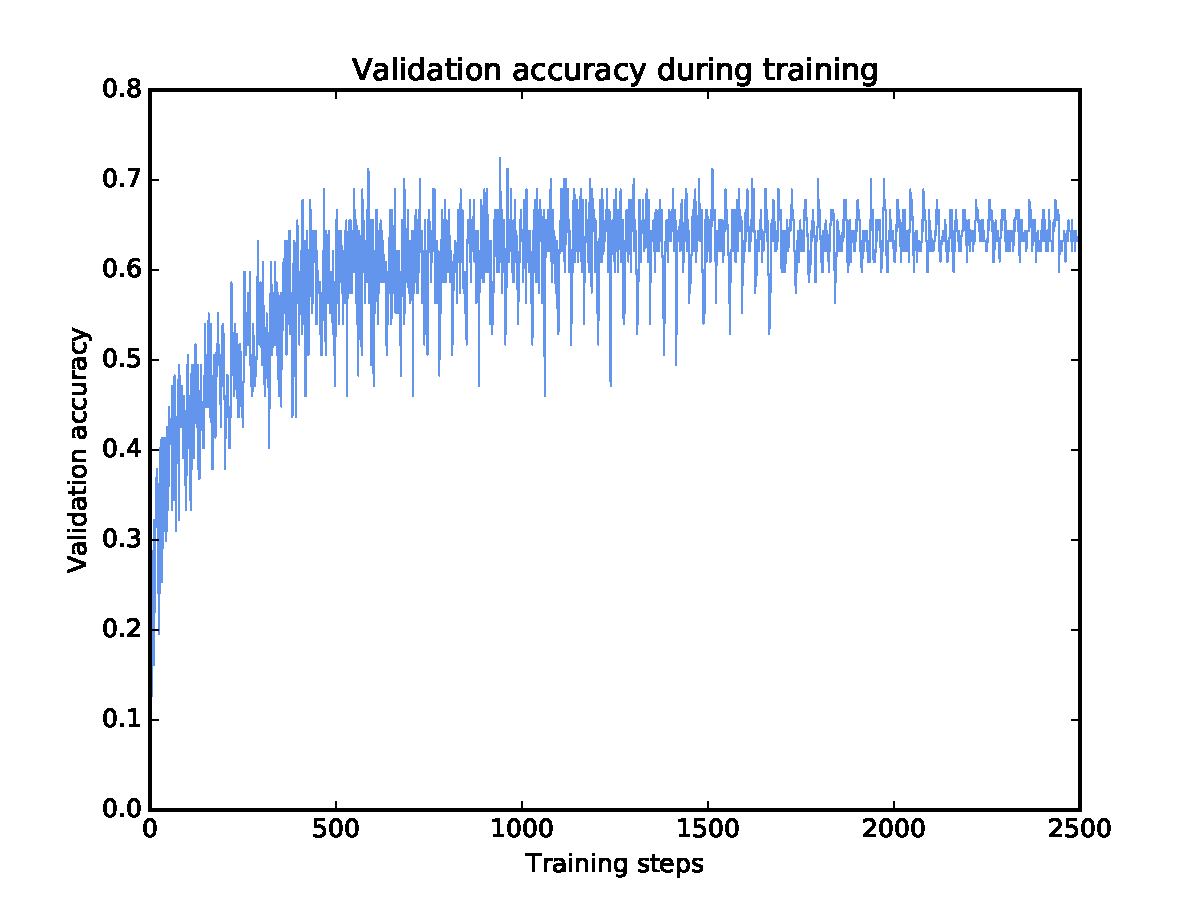
\includegraphics[width=4.5in]{img/2-4-4-validation-acc-new.pdf}
   \caption{Validation error of one realization of our convolutional network
   (with all hyperparameters unchanged from their original values)
   during training.}
   \label{fig:2-4-4-validation-acc}
\end{figure*}

Notice that after 1000 training steps,
validation accuracy fails to improve further.
However, validation accuracy
does not significantly \emph{decrease}
as we continue to train our model,
suggesting that overfitting (if it is occurring at all)
is not negatively impacting our results.

In summary, none of our regularization schemes
was particularly effective in improving validation accuracy.



\subsection{Architectural variations}

We also tried varying our network architecture,
rather than just tweaking training parameters
(e.g. weight regularization, dropout).

%    Report which changes led to
%    the biggest increases and decreases in performance.
%    In particular,
%    what is the effect of making the convolutional layers have
%    a) a larger filter size,

\subsubsection{Filter sizes, stride}

We tested larger and smaller filter sizes
on each convolutional layer.
We first tried changing the filter sizes on both layers simultaneously,
leaving other hyperparameters fixed.
Filters larger than $5\times 5$ performed just as well,
while smaller filters performed significantly worse.
More novel filter size combinations
did not yield any improvement either.

%We present some of our findings
%in Figure~\ref{fig:filter-size-experiment}.
%
%\begin{figure*}[t]
%   \centering
%   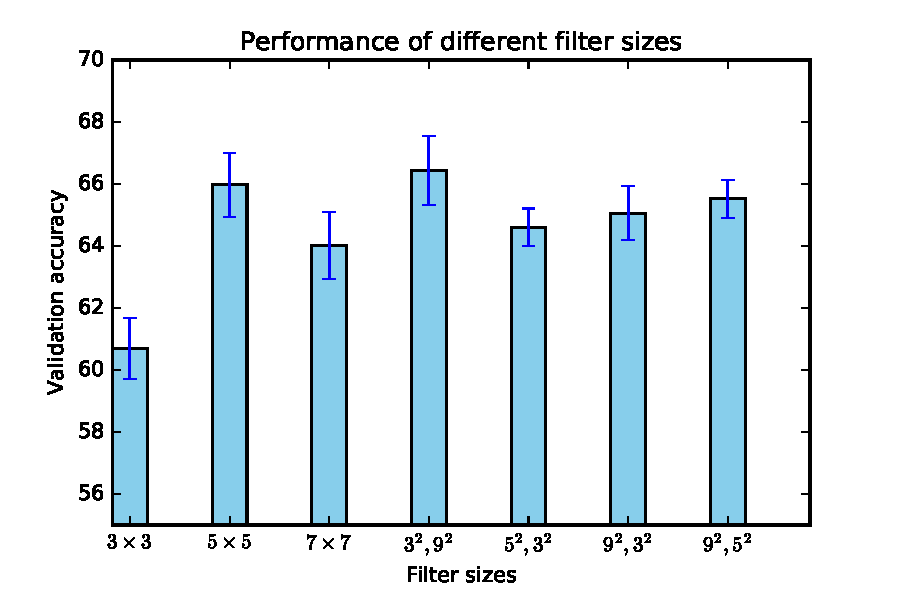
\includegraphics[width=4in]{img/2-5-filter-size-acc.pdf} 
%   \caption{Mean validation accuracies for various filter size choices (each tested $n=10$ times).
%       Error bars denote standard error of the mean.}
%   \label{fig:filter-size-experiment}
%\end{figure*}

%\begin{center}
%    \begin{tabular}{c|cc}
%        Filter sizes & Train $\pm 1 \sigma$ (\%) & Validation $\pm 1 \sigma$\\\hline
%        $3\times 3$ & $95.00 \pm 1.67$ & $60.69 \pm 0.98$ \\
%        $5\times 5$ & $100.00 \pm 0.00$ & $65.98 \pm 1.03$ \\
%        $7\times 7$ & $100.00 \pm 0.00$ & $64.02 \pm 1.07$ \\
%        $3^2$ then $9^2$ & $100.00 \pm 0.00$ & $66.44 \pm 1.12$ \\
%        $5^2$ then $3^2$ & $98.00 \pm 2.00$ & $64.60 \pm 0.61$ \\
%        $9^2$ then $3^2$ & $100.00 \pm 0.00$ & $65.06 \pm 0.88$ \\        
%        $9^2$ then $5^2$ & $100.00 \pm 0.00$ & $65.52 \pm 0.62$
%    \end{tabular}
%\end{center}

%    b) a larger stride and
We tried varying the strides on our convolutional layers as well.
No setting we tried produced statistically significant improvement
over our baseline $5\times 5$ filters with stride $2$.


%    c) greater depth?
\subsubsection{Depth}

Finally, we varied the number of feature maps
we used at each layer.
For this section,
we included $2\times 2$ max-pooling layers with stride 2
after each convolutional layer.
(We found that pooling significantly improved results.)

Holding the depths of the two convolutional layers equal,
increasing the depth significantly improved validation accuracies
(Figure~\ref{fig:2-5-conv-depth-val-acc}).
At depth 45, we achieved a mean validation accuracy of $70.5 \pm 0.9\%$,
which was statistically significantly greater
than our baseline (depth~15) of $64.8 \pm 1.1\%$
(Student's $t$-test, $p=0.001$).

\begin{figure*}[t]
   \centering
   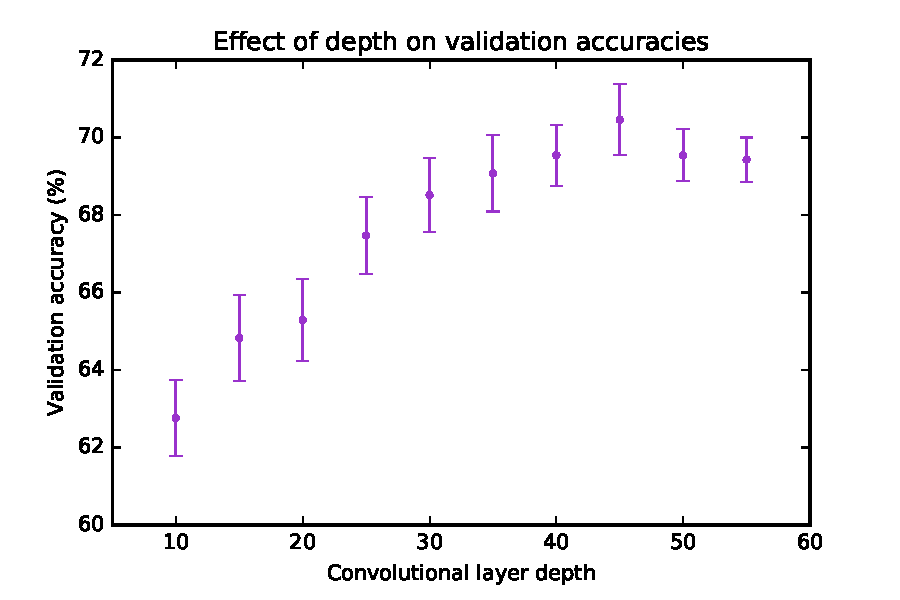
\includegraphics[width=4.5in]{img/2-5-conv-depth-val-acc.pdf}
   \caption{Mean validation accuracies (with standard errors of the means)
       of convolutional networks with equal depth at both convolutional layers.}
   \label{fig:2-5-conv-depth-val-acc}
\end{figure*}

Near-perfect training accuracies in each of these tests
suggested some degree of overfitting.


%    How does a pyramidal-shaped network
%    in which the feature maps gradually decrease in height and width
%    but increase in depth
%    compare to a flat architecture,
%    or one with the opposite shape?

We also varied depths independently.
We tested ``pyramidal" architectures
in which the second layer had a larger depth
compared with the first;
we also tried the reverse architecture.
No such architecture performed better
than the best architecture we found when
we varied the depths in lockstep (depths 45 and 45).


\subsection{Invariance}

Further experimentation with training parameters
failed to improve upon
the optimal architecture from the previous section
(depths 45 and 45, with pooling layers),
which we took as our best model.
We tested it on transformed versions of the validation data.

We present the results of one test here:
\begin{center}
    \begin{tabular}{c|c}
        transformation & accuracy (\%) \\\hline
        none & 71.26 \\
        translated & 37.93\\
        brightened & 35.63\\
        darkened & 59.77\\
        high contrast & 35.63 \\
        low contrast &59.77\\
        flipped & 44.83\\
        inverted & 9.20
    \end{tabular}
\end{center}
Our model was relatively insensitive
to decreases in contrast and brightness;
it was modestly more sensitive to increases in the same.
Flipping the images also appreciably decreased classification accuracy,
suggesting that our model learned directional features from the paintings.

On the other hand,
our network was very sensitive to color inversion,
suggesting that it learned features
related to different artists' choice of color.

\end{multicols}

\end{document}

